During this second year another four territorial PoPs have been raised and made operative, amounting to a total of eight territorial and the concentration one (Telvent -Barcelona) operational. Figure~\ref{fig:pop_weathermap} shows their distribution on the map. So far all the territorial PoPs are connected to the concentration one via XOC connections\footnote{The prices can be found at \url{http://www.xarxaoberta.cat/en/prices}.}.

\begin{figure}[H]
  \centering
  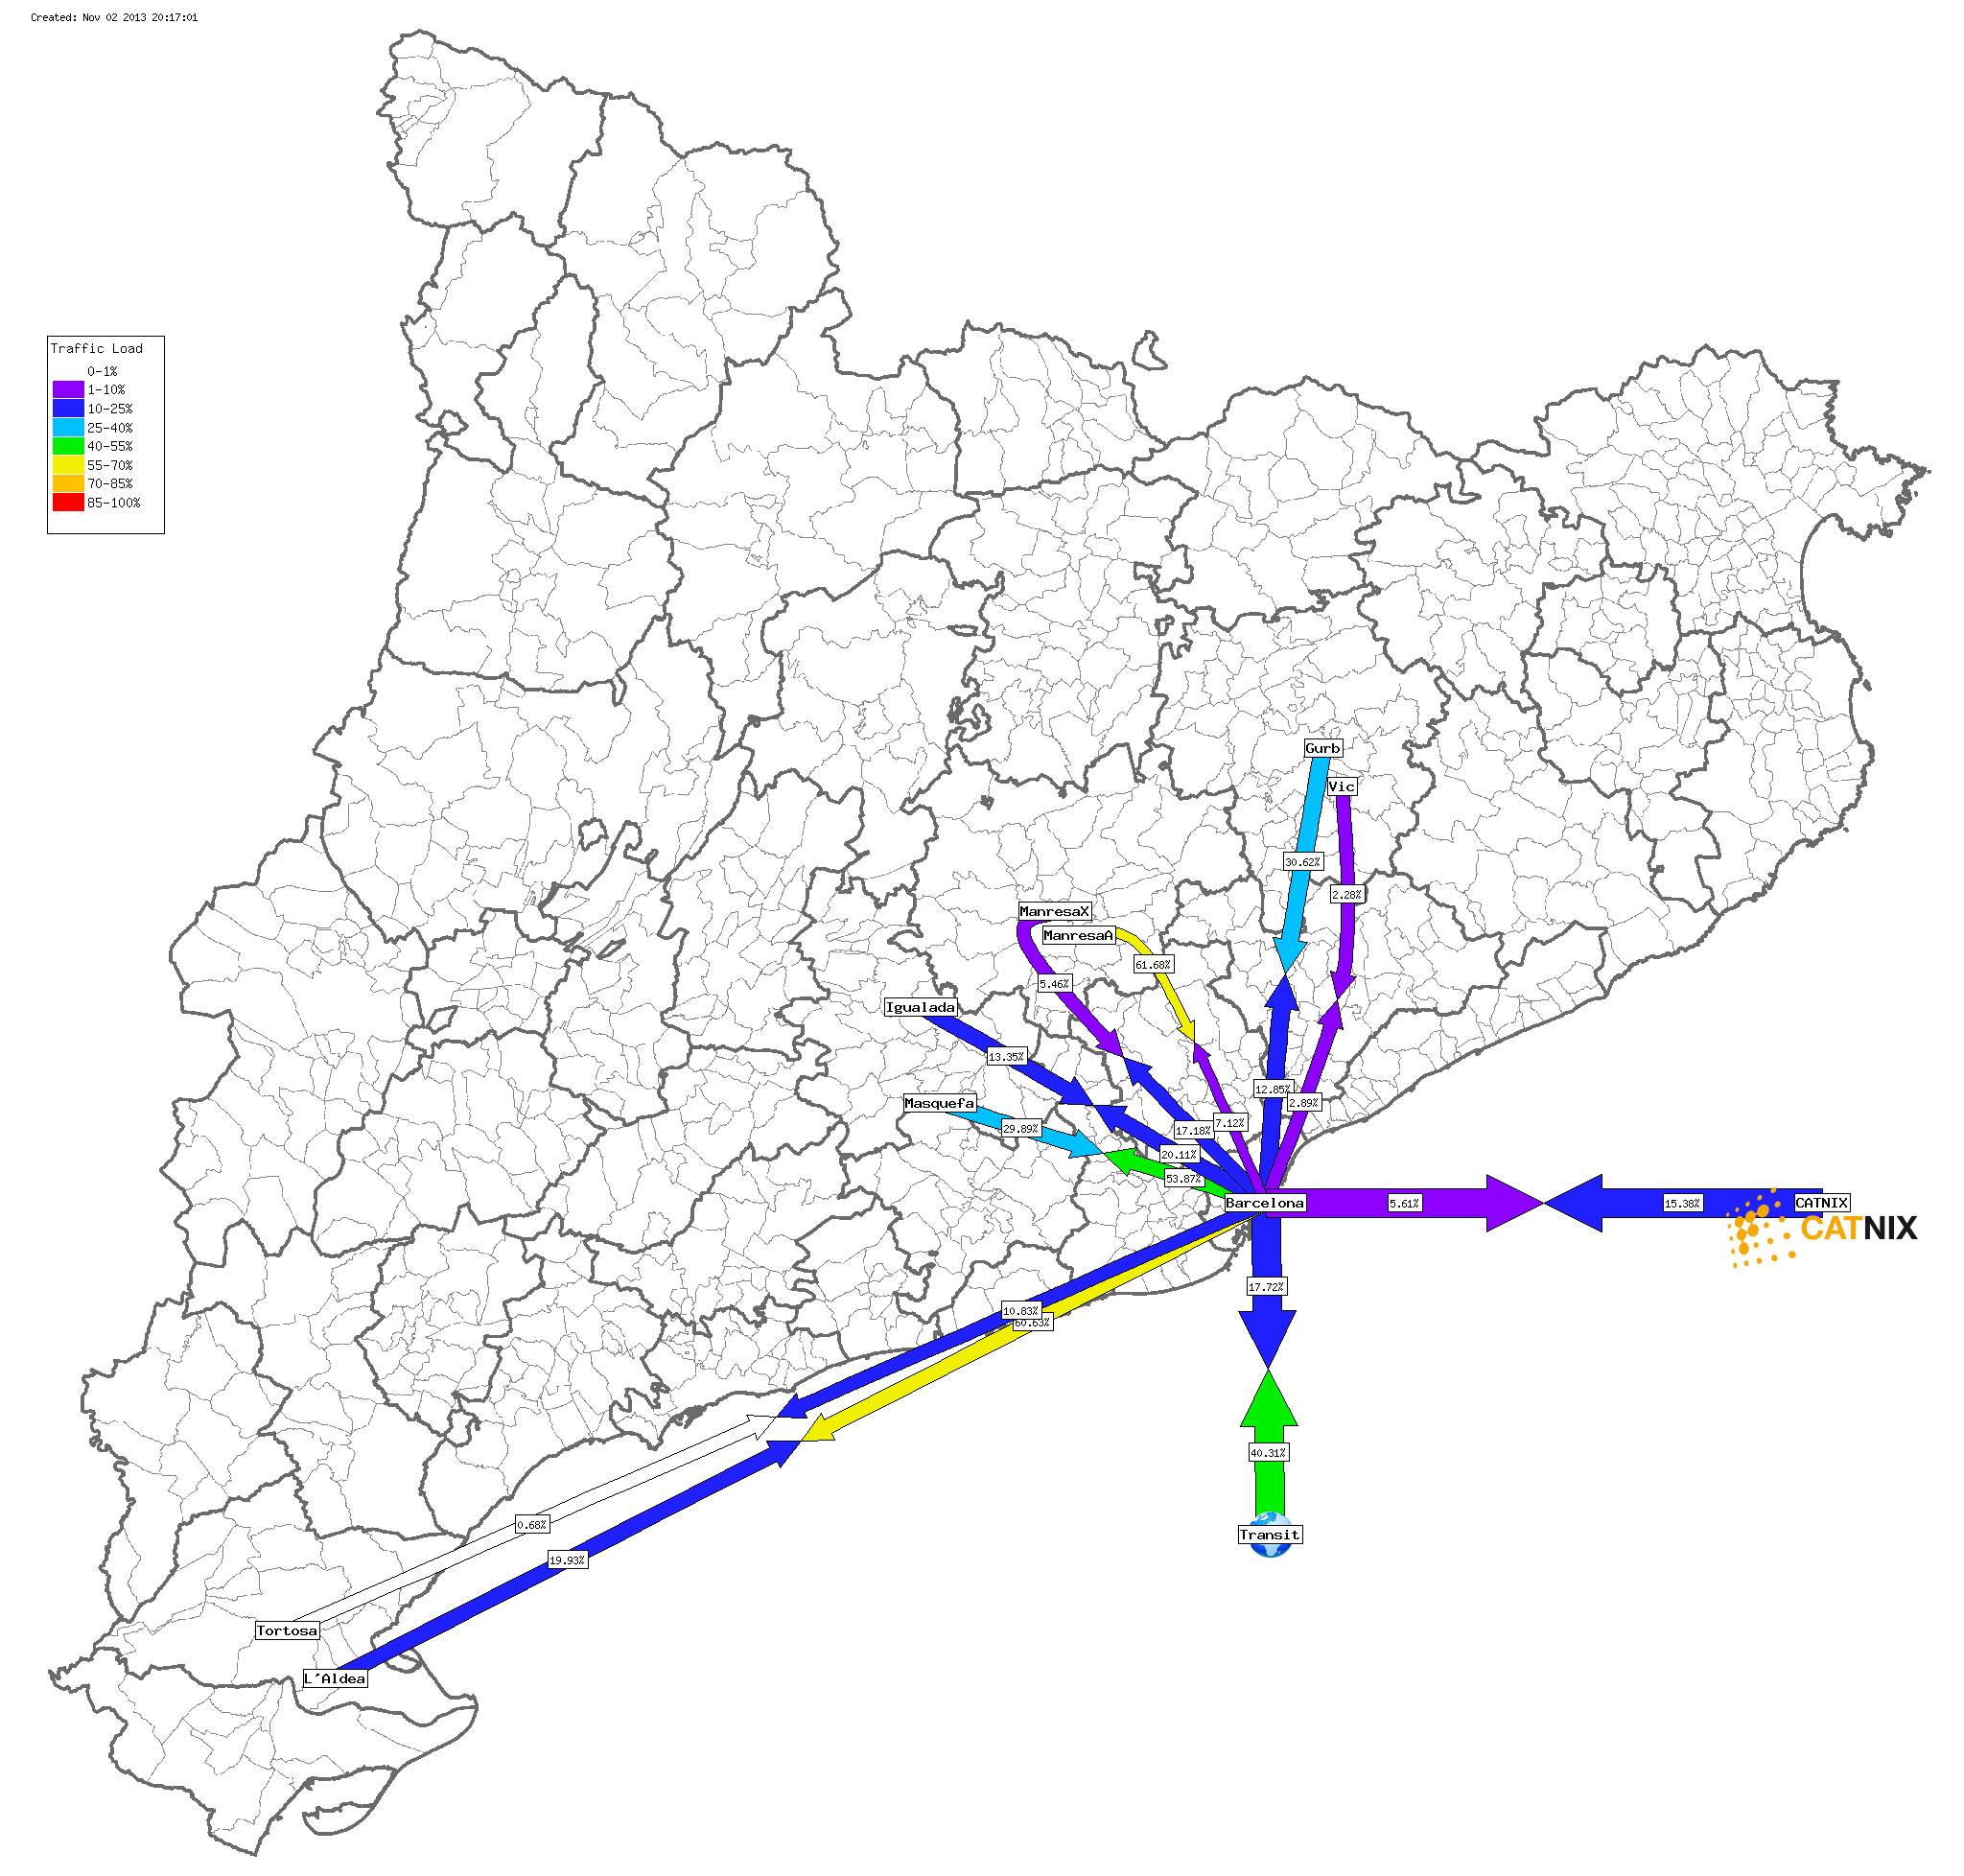
\includegraphics[width=0.95\linewidth]{sect3/figures/weathermap.png} 
  \caption[Guifi.net fiber POPs network map 2013]{Guifi.net fiber POPs network map 2013.}
  \label{fig:pop_weathermap}
\end{figure}

With respect to the IXs operation, the following improvements have been applied during this year:
\begin{itemize}
  \item The management system has been notably enhanced.
  \item A new monitoring development was launched in June 2013 (consequently, most of the traffic graphs shown in the document stars at that moment).
  \item The implementation of a more efficient accounting system has been started and it is expected to be fully operational in 2014. This system will make the ISPs' theshowback/chargeback more accurate and fair.
  \item The equipment of most of the PoPs has been completed and updated.
\end{itemize}

As an example of the current state of the art of the PoPs Figure~\ref{fig:telvent_diagram} shows Telvent's PoP at wiring level.

\begin{figure}[H]
  \centering
<<<<<<< HEAD:D_5_4_2_report_on_pilots_on_fiber_deployment_b/pops/pops.tex
  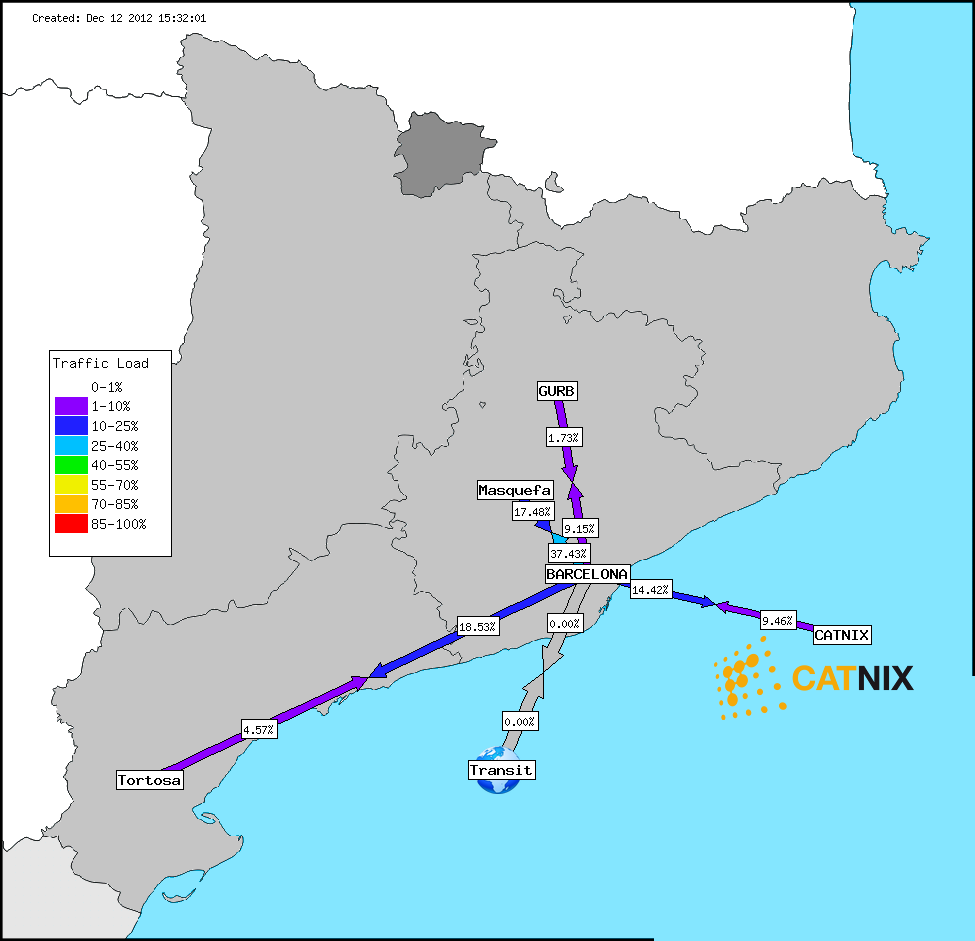
\includegraphics[scale=.35]{pops/figures/pops_network_map.eps} 
  \caption{Guifi.net fiber POPs network map}
  \label{fig:fibre_map}
=======
  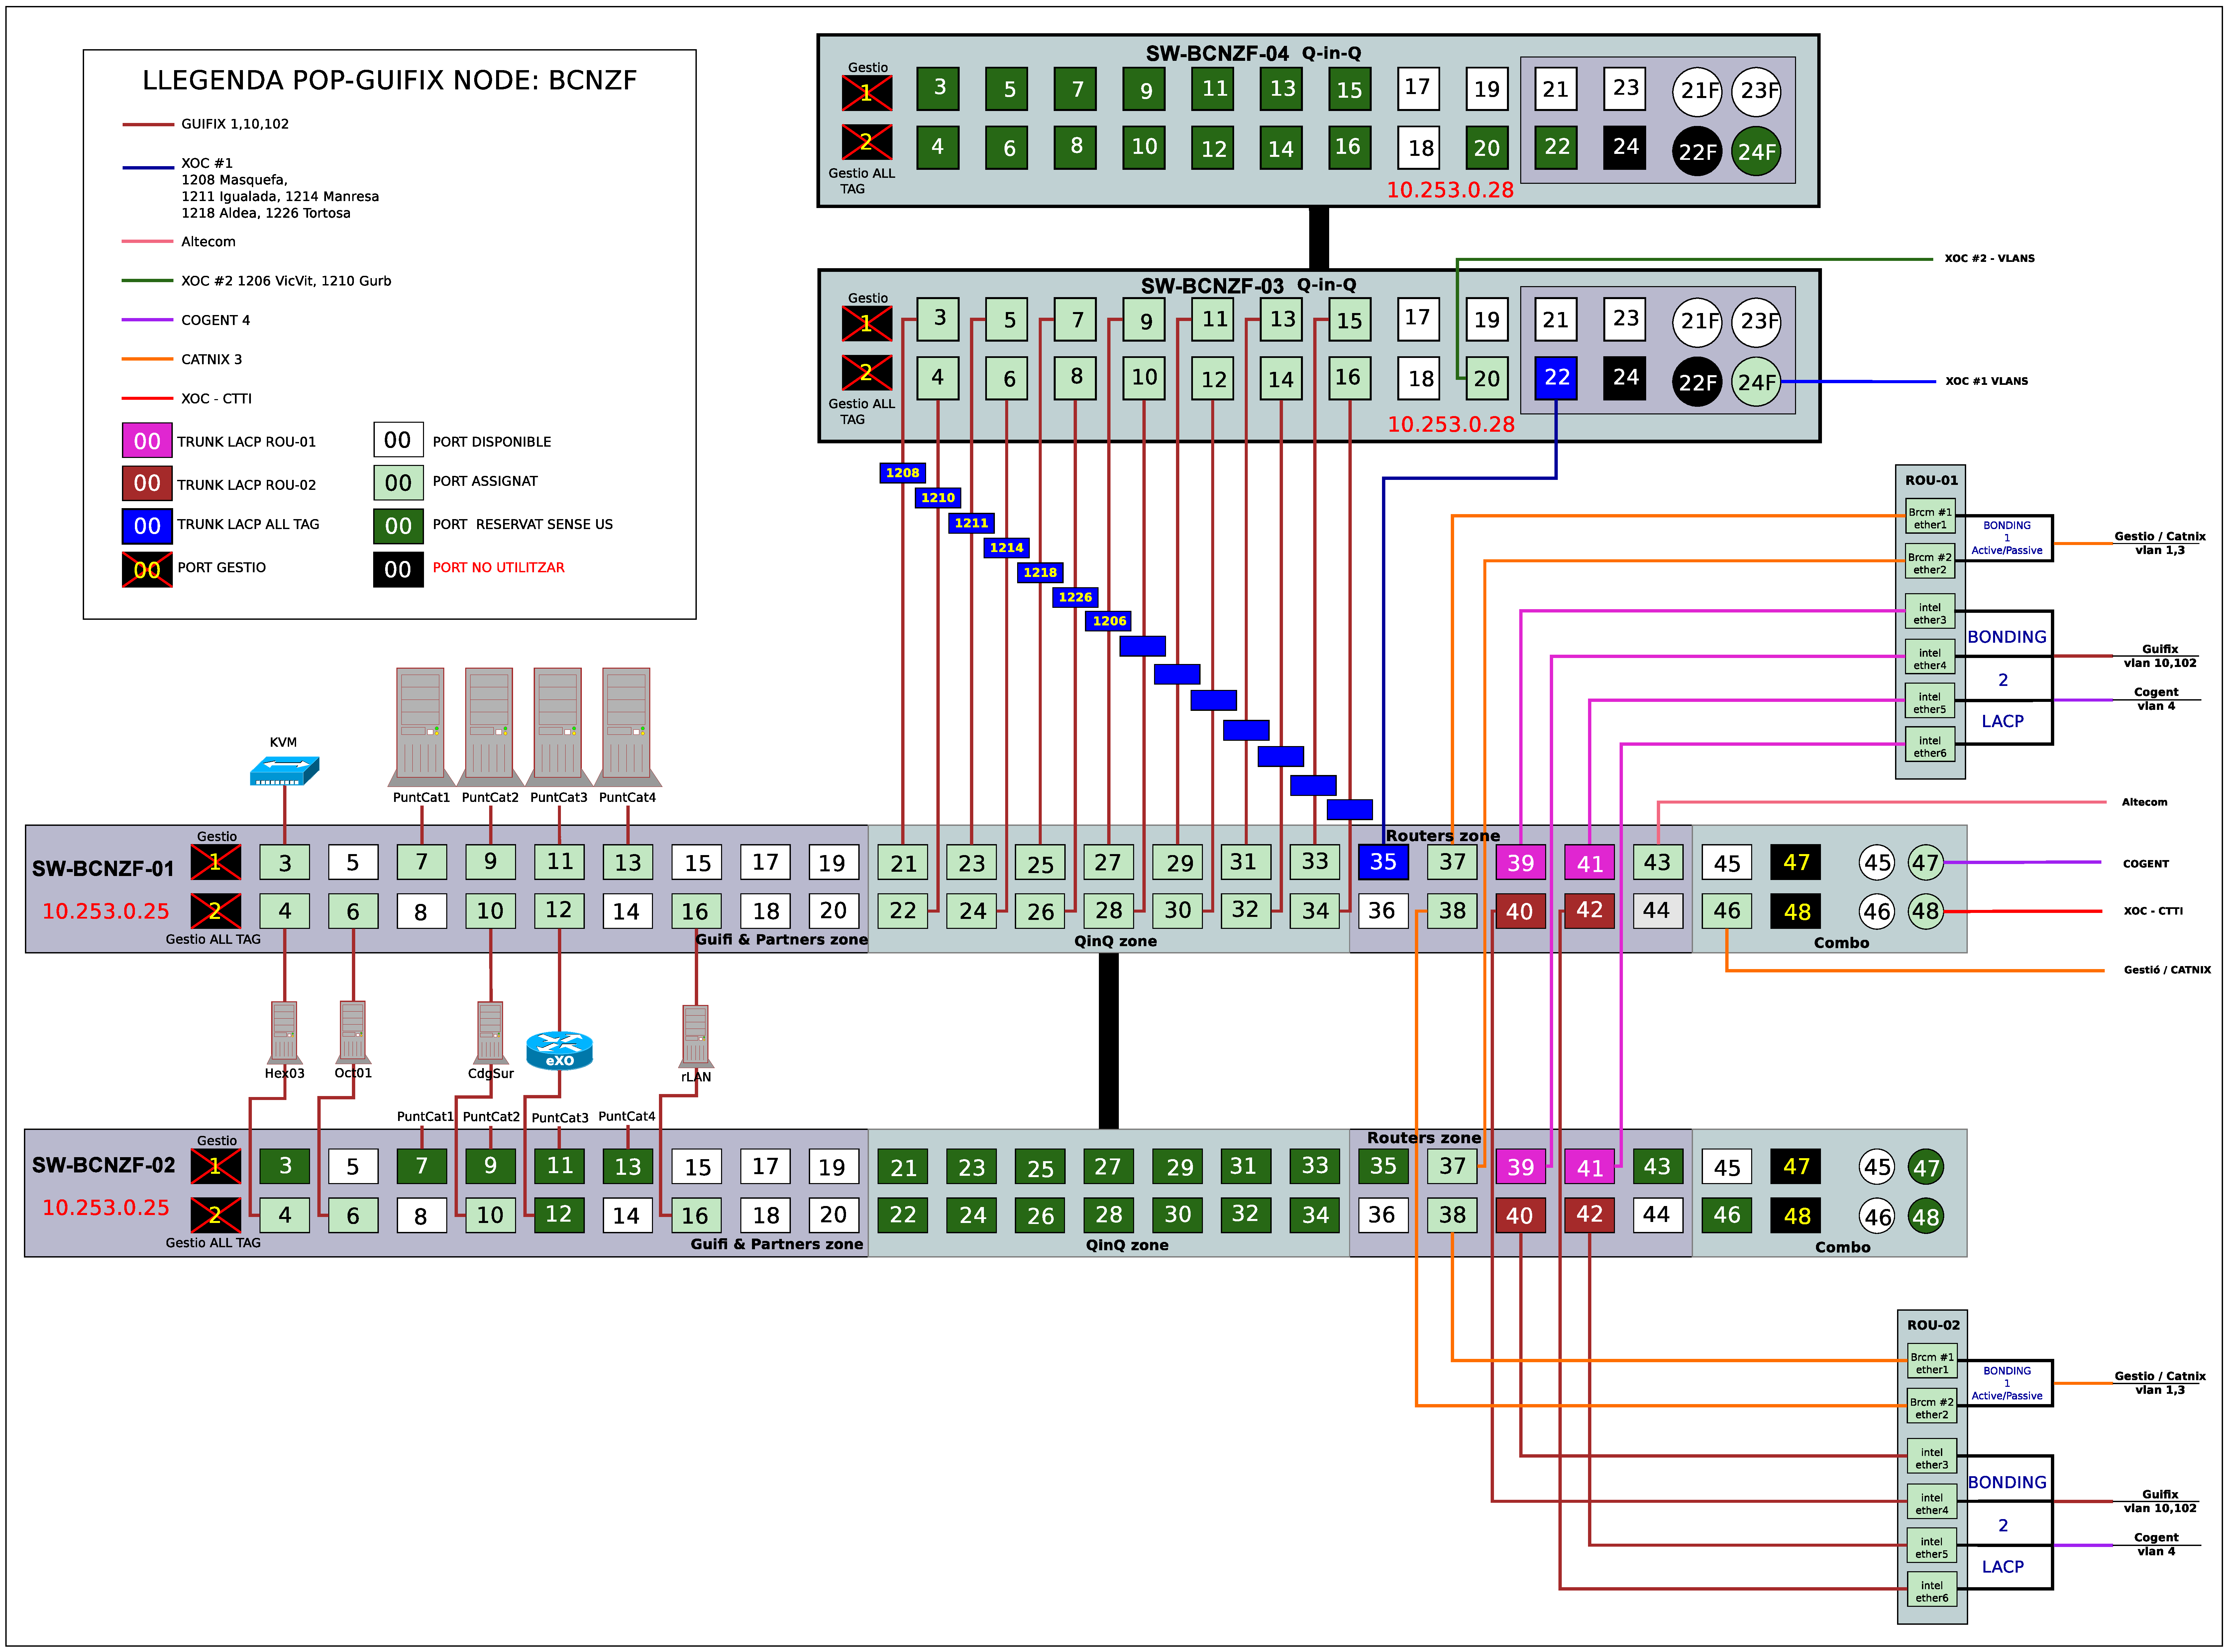
\includegraphics[width=0.95\linewidth]{sect3/figures/telvent_diagram.eps} 
  \caption[Telvent network diagram]{Telvent network diagram Oct. 2013.}
  \label{fig:telvent_diagram}
>>>>>>> rbaig/master:D_5_4_2_report_on_pilots_on_fiber_deployment_b/sect3/pops.tex
\end{figure}


During this period the CATNIX (the Catalan exchange point) peering process has been completed. As a result, the guifi.net Foundation is peering with all the other CATNIX members with the exception of the big ISPs (the Telefonica -the incumbent, Ono and BT). These ISPs have not shown any interest in peering with us.

Figure~\ref{fig:catnix_transit} shows the evolution of the peering traffic and Figure~\ref{fig:cogent_transit} shows the traffic to Cogent (our internet carrier). A second carrier is expected to be hired in the coming weeks, essentially to have a redundant internet access but also to anticipate the bandwidth demand.

\begin{figure}[H]
  \centering
<<<<<<< HEAD:D_5_4_2_report_on_pilots_on_fiber_deployment_b/pops/pops.tex
    \begin{tabular}{cc}
      \resizebox{70mm}{!}{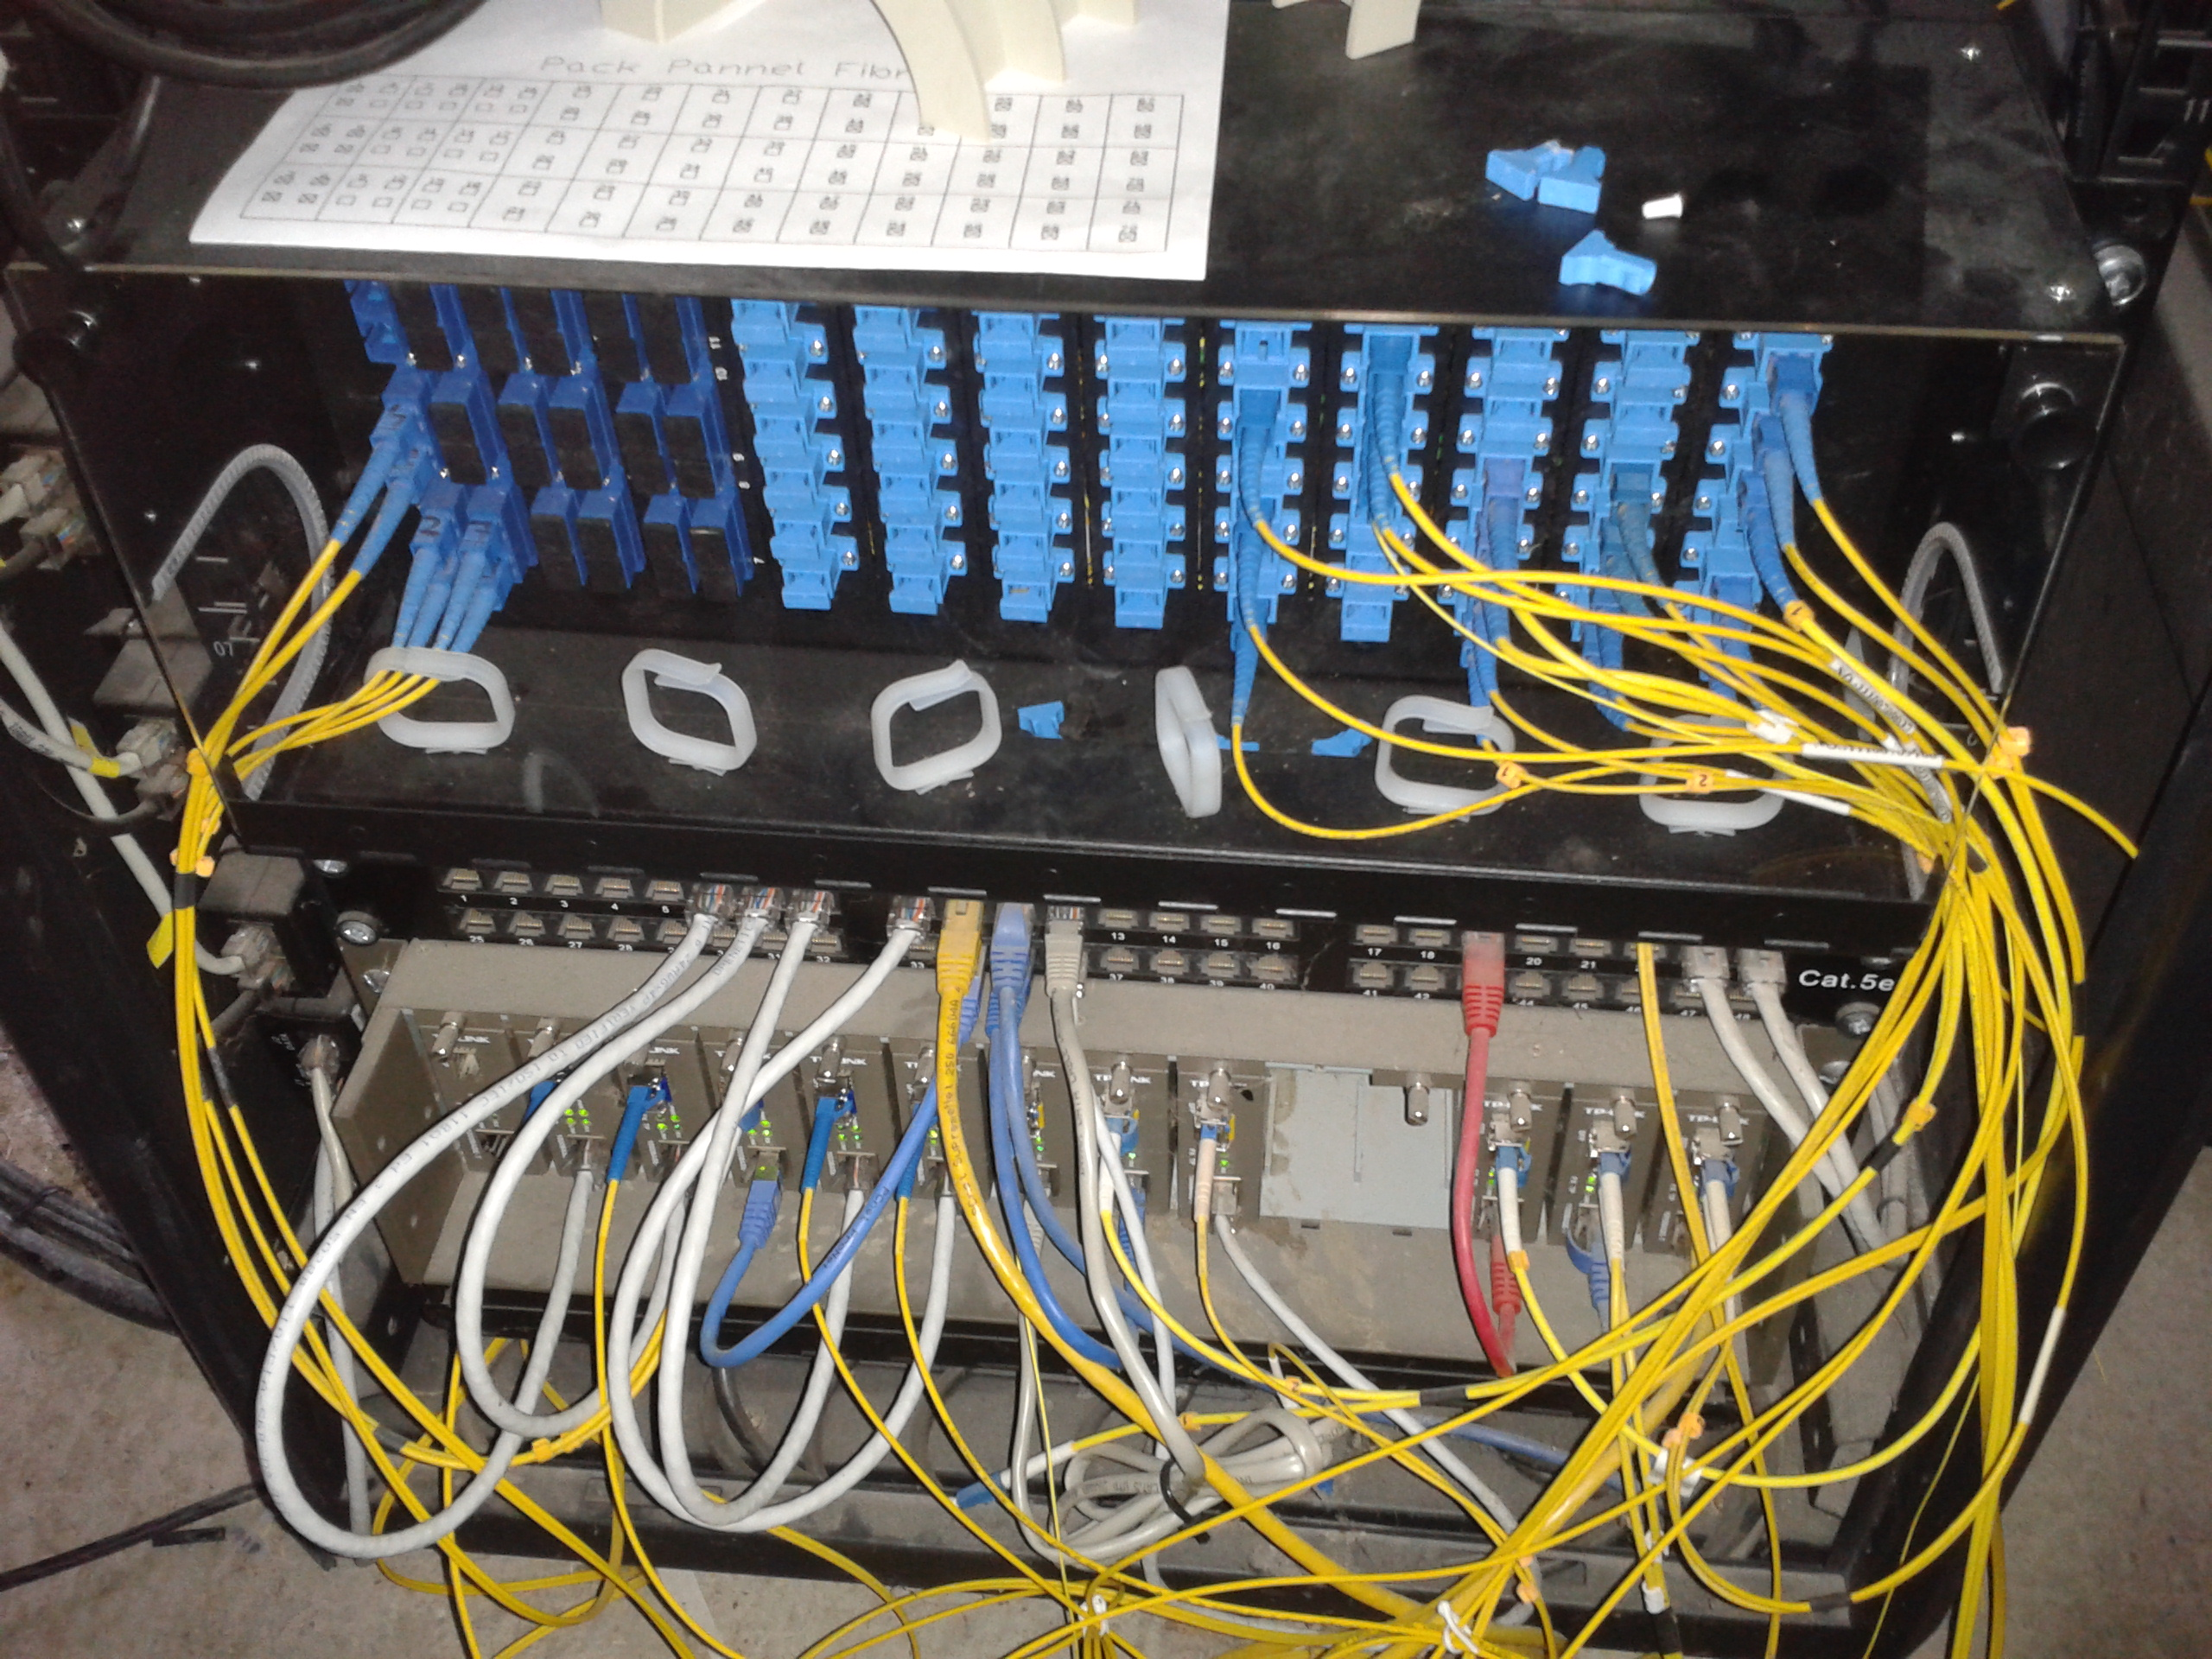
\includegraphics{pops/figures/gurb_rack1.eps}} &
      \resizebox{70mm}{!}{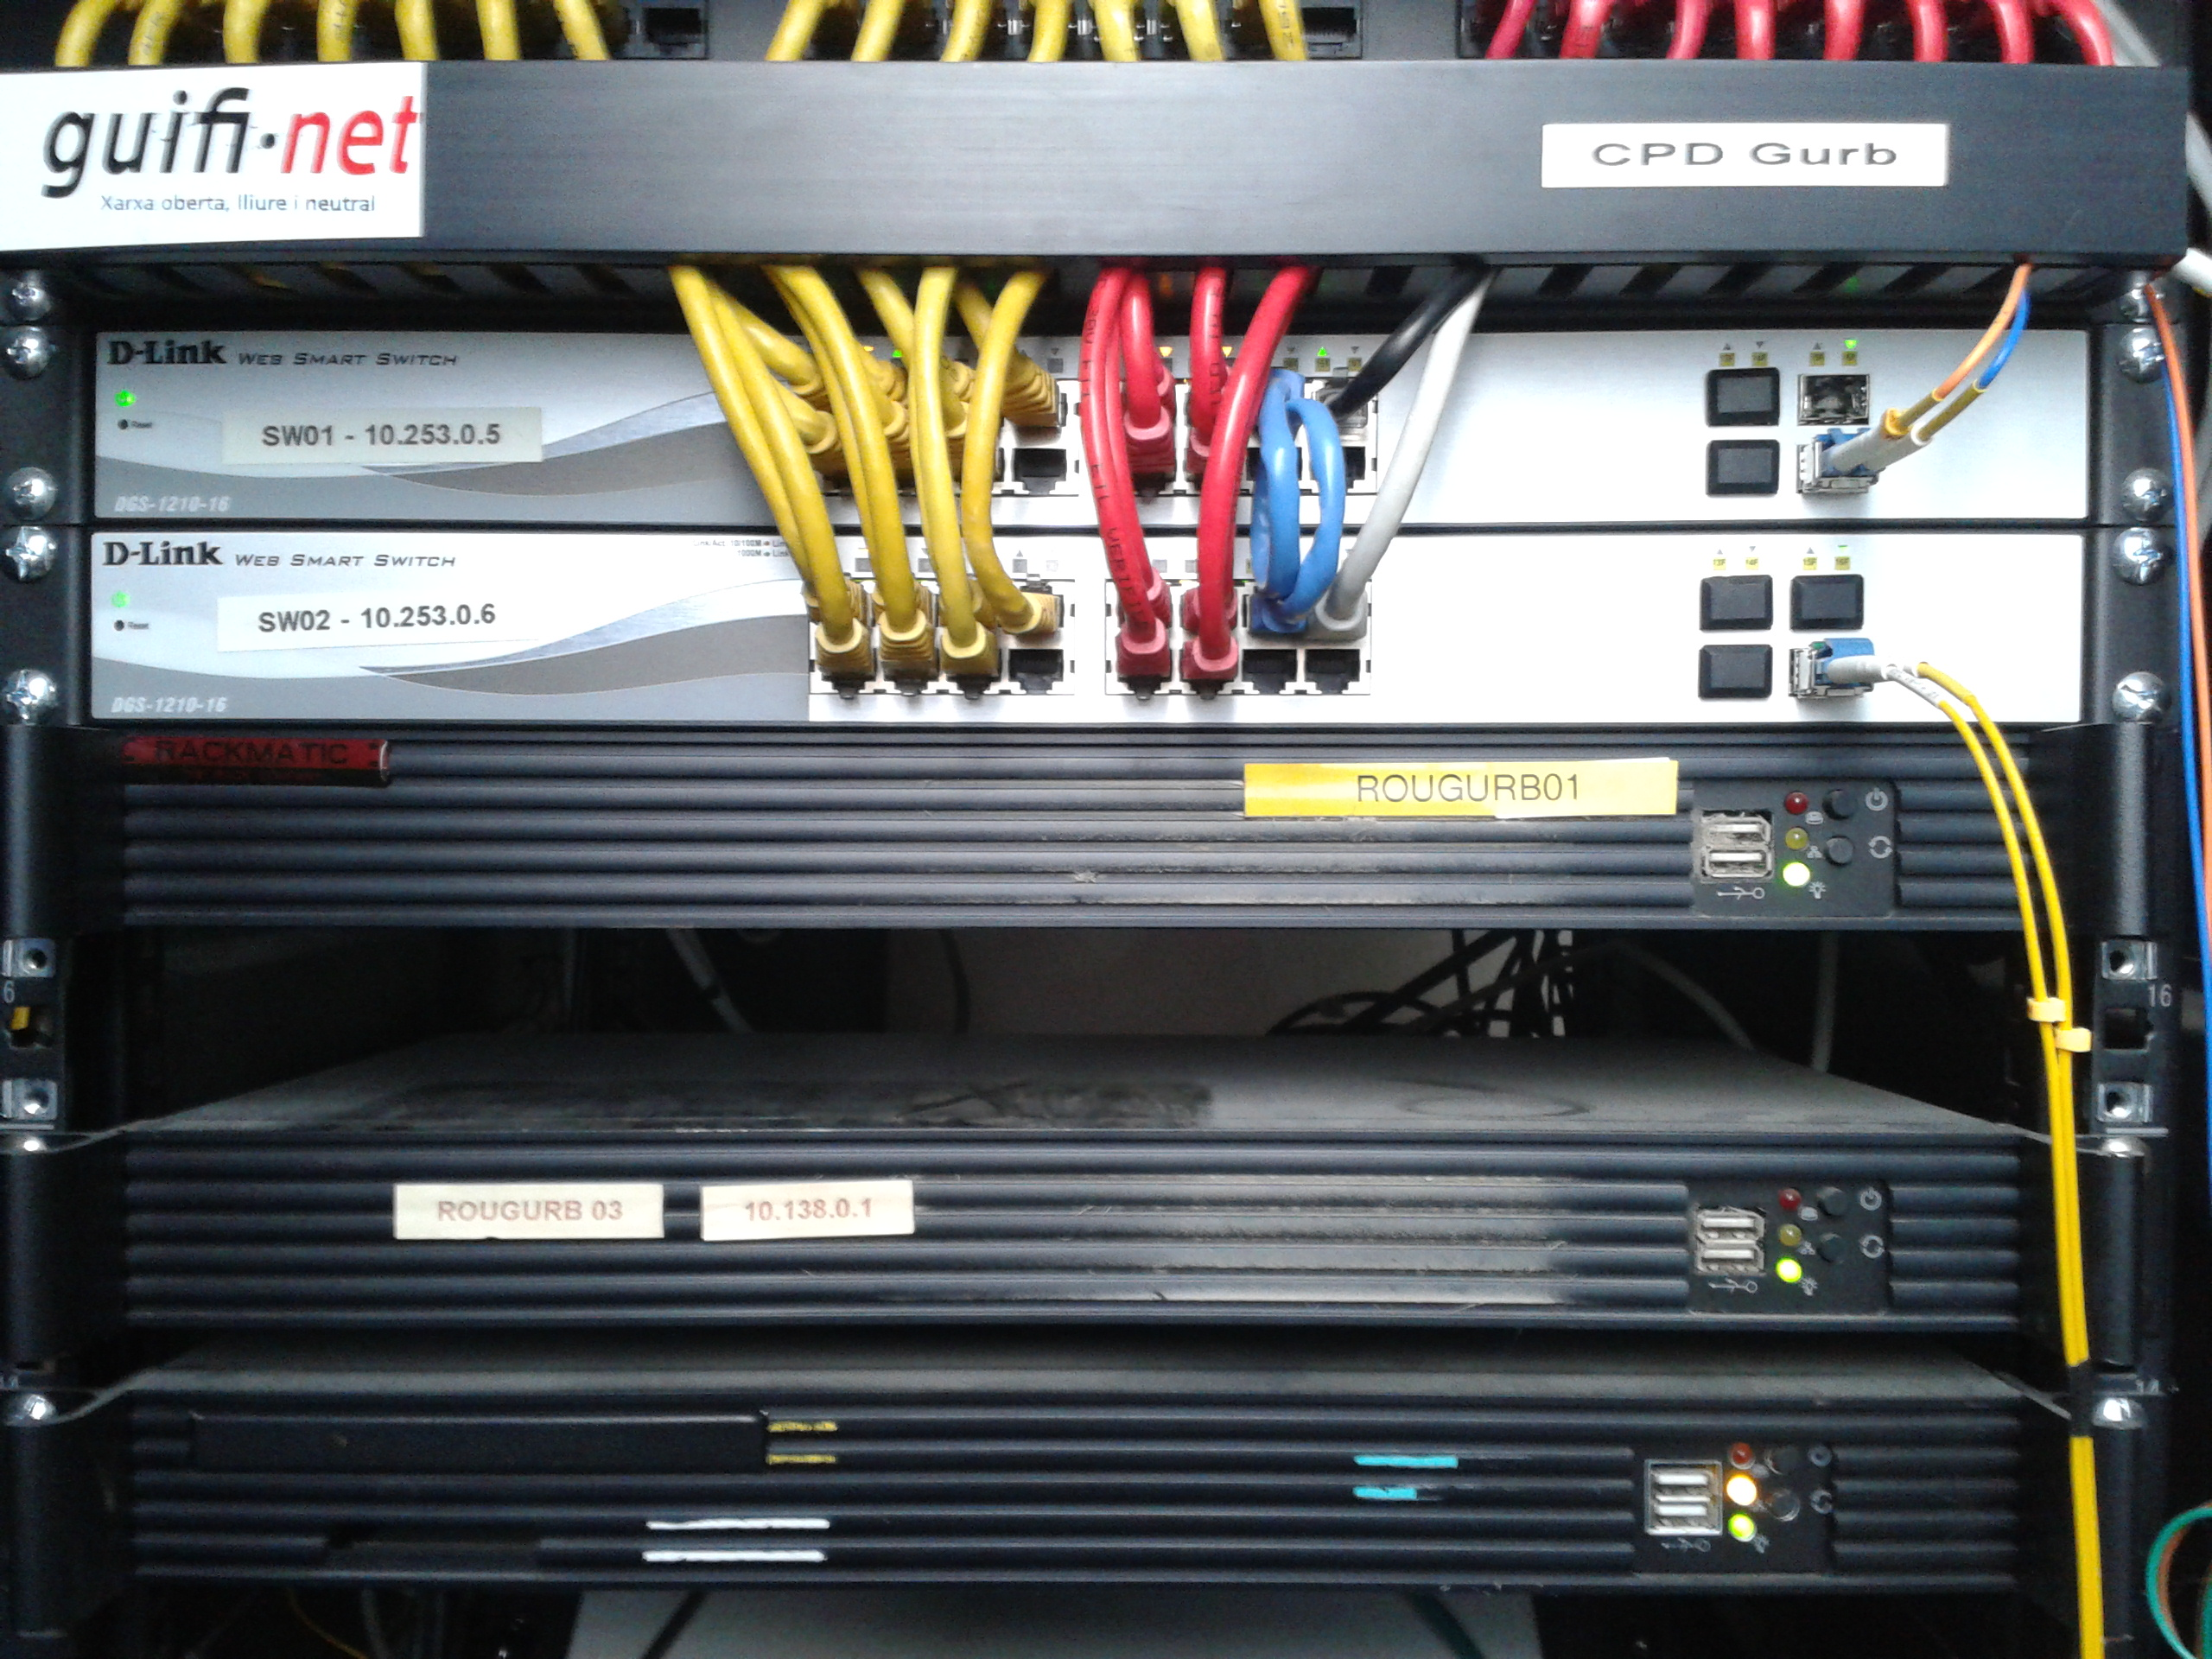
\includegraphics{pops/figures/gurb_rack2.eps}} \\
    \end{tabular}
  \caption{Gurb's POP detailed pictures. On the right the OF terminations. On the left the routers.}
  \label{fig:grub_rack}
=======
  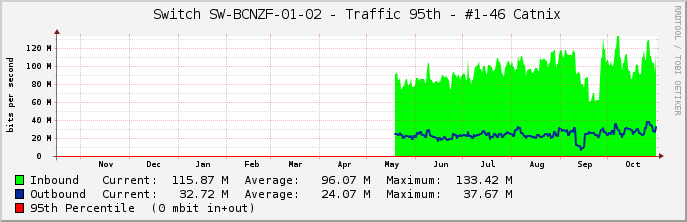
\includegraphics[width=0.95\linewidth]{sect3/figures/catnix.png} 
  \caption[CATNIX traffic 2013]{CATNIX traffic 2013.}
  \label{fig:catnix_transit}
>>>>>>> rbaig/master:D_5_4_2_report_on_pilots_on_fiber_deployment_b/sect3/pops.tex
\end{figure}

\begin{figure}[H]
  \centering
<<<<<<< HEAD:D_5_4_2_report_on_pilots_on_fiber_deployment_b/pops/pops.tex
  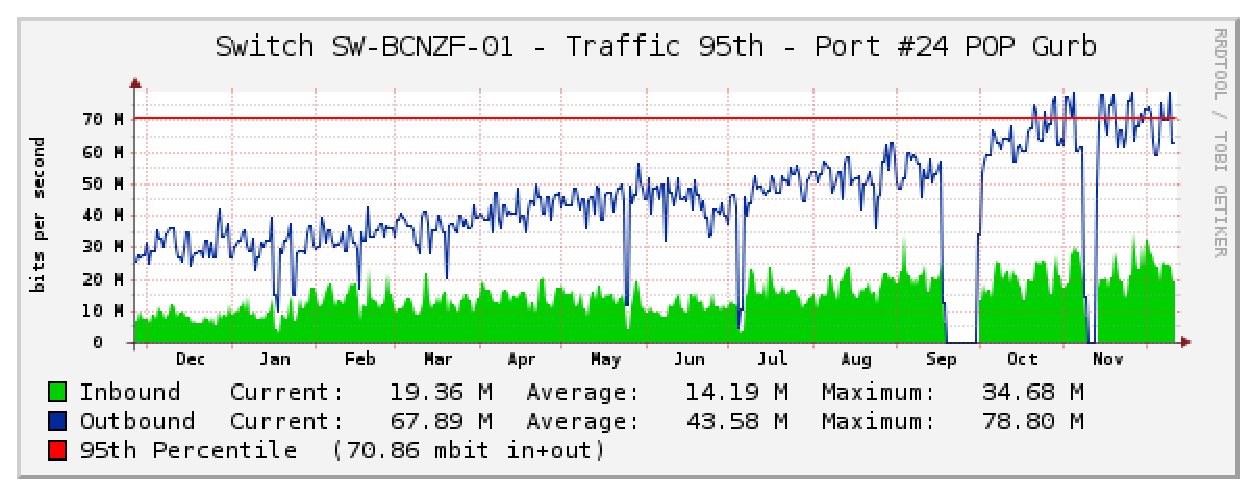
\includegraphics[scale=.65]{pops/figures/gurb_network_load_year.eps} 
  \caption{Gurb's POP network load (year 2012).}
  \label{fig:gurb_net_load}
=======
  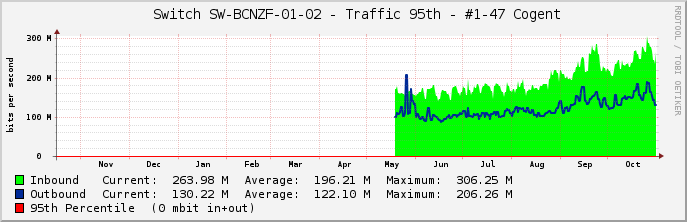
\includegraphics[width=0.95\linewidth]{sect3/figures/cogent.png} 
  \caption[Cogent traffic 2013]{Cogent traffic 2013.}
  \label{fig:cogent_transit}
>>>>>>> rbaig/master:D_5_4_2_report_on_pilots_on_fiber_deployment_b/sect3/pops.tex
\end{figure}

\FloatBarrier
\subsection{Pilot's POPs}
\label{pop_pilots}


\FloatBarrier
<<<<<<< HEAD:D_5_4_2_report_on_pilots_on_fiber_deployment_b/pops/pops.tex
\subsubsection{Telvent-Barcelona}

Telvent-Barcelona is a commercial data center\footnote{\url{http://www.telvent.es/en/}} placed in an industrial park of Barcelona. It hosts the CATNIX\footnote{\url{http://www.catnix.net}}, the Internet exchange point (IX) of Catalonia, a physical infrastructure provided by the Catalan government. IXs are critical for the Internet since they are meant to let the network operators exchange their information and connect their networks (autonomous systems). 

On the one hand, as be shown in Figure \ref{fig:fibre_map}, all guifi.net POPs are linked to TELVENT-Barcelona. On the other hand, guifi.net connects to the Internet through this POP.

guifi.net Foundation operates it's own backbone infrastructure using the ASN 49835 (Autonomous System Number). 
An open peering policy is followed to establish peering sessions with all potential partners. Figure~\ref{fig:catnix_net_load} shows the total peering traffic of guifi.net CATNIX port\footnote{To be a CATNIX members must have at least one public ASN and one public IP block. Guifi.net is a Local Internet Registry (LIR) since it is a RIPE-NCC member, and has its own ASN numbers and IPv4 and IPv6 blocks.}. Additionally guifi.net Foundation has an Internet Gigabit uplink contracted with Cogent\footnote{\url{http://www.cogentco.com/en/}}. Figure~\ref{fig:cogent_load} . All guifi.net Foundation routers and servers are allocated in a 22U rack in Telvent-Barcelona, shown in Figure~\ref{fig:telvent_rack}. 


Figure \ref{fig:telvent_scheme} shows a connection scheme (layer 2) of the hardware used for the CATNIX POP. 
The first port of the switch SW-03 is the optical fiber which brings the data from the other POPs. As can be seen each
of them use a separate VLAN. The seventh port of the second switch is the connection with the carrier to reach the Internet.
And the eight is connected to the CATNIX infrastructure where the exchange of data with other ISPs and networks is possible. 


The Telvent-Barcelona Foundation resources are shared with other partners, such as puntCat\footnote{\url{http://www.domini.cat/}}, the Catalan Top-Level Domain (TDL), which is currently using half of the space available.

\begin{figure}[htbp]
  \centering
  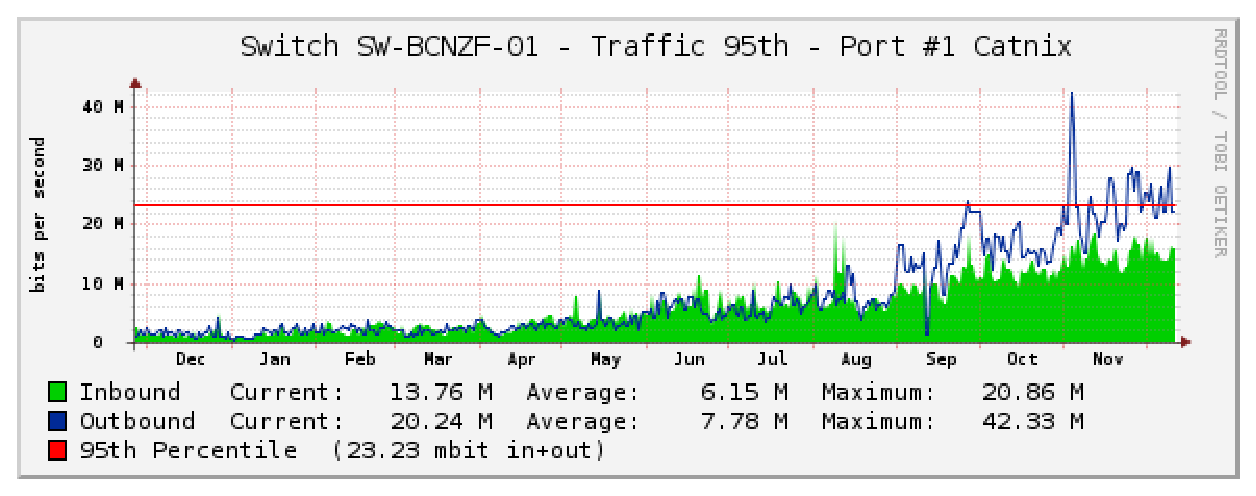
\includegraphics[scale=.65]{pops/figures/catnix_network_load_year.eps} 
  \caption{Telvent-Barcelona's POP network load (year 2012).}
  \label{fig:catnix_net_load}
\end{figure}
=======
\subsubsection{Gurb}
\label{pop_gurb}
>>>>>>> rbaig/master:D_5_4_2_report_on_pilots_on_fiber_deployment_b/sect3/pops.tex

This PoP has been operative since 2010. This year the power supply system has been improved by adding a back-up power supply. Also the electronic equipment has been significantly extended to accommodate the necessities deriving from Gurb's OF pilot deployment and other connections. Firgure~\ref{fig:gurb_transit} shows the transit of this PoP.

\begin{figure}[H]
  \centering
<<<<<<< HEAD:D_5_4_2_report_on_pilots_on_fiber_deployment_b/pops/pops.tex
  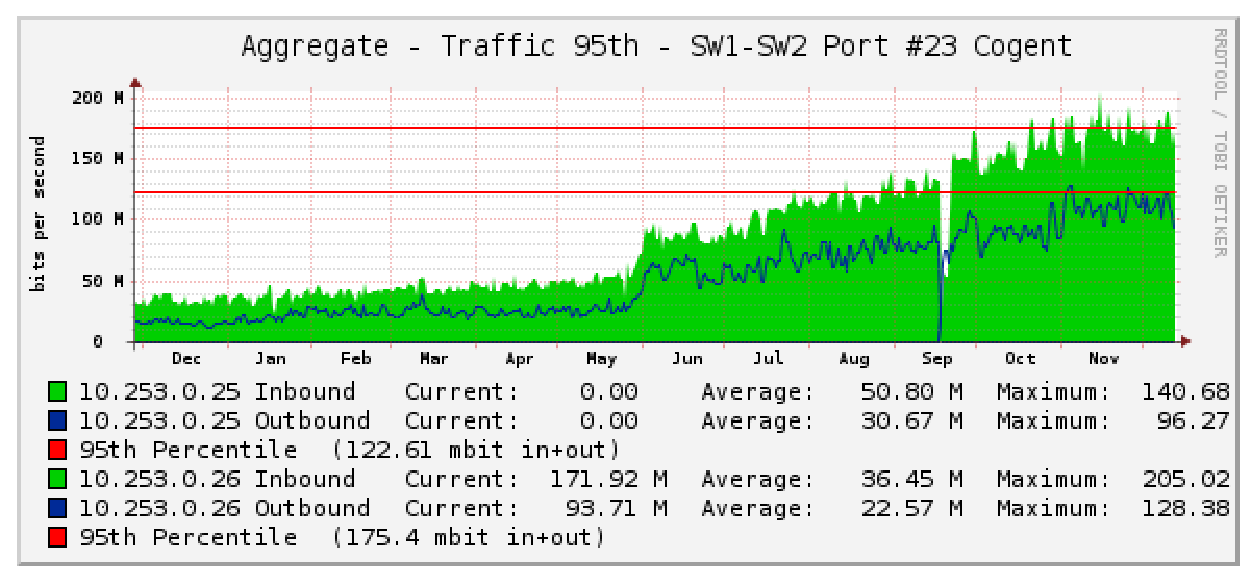
\includegraphics[scale=.65]{pops/figures/cogent_network_load2.eps} 
  \caption{Internet uplink load (year 2012).}
  \label{fig:cogent_load}
\end{figure}


\begin{figure}[htbp]
  \centering
  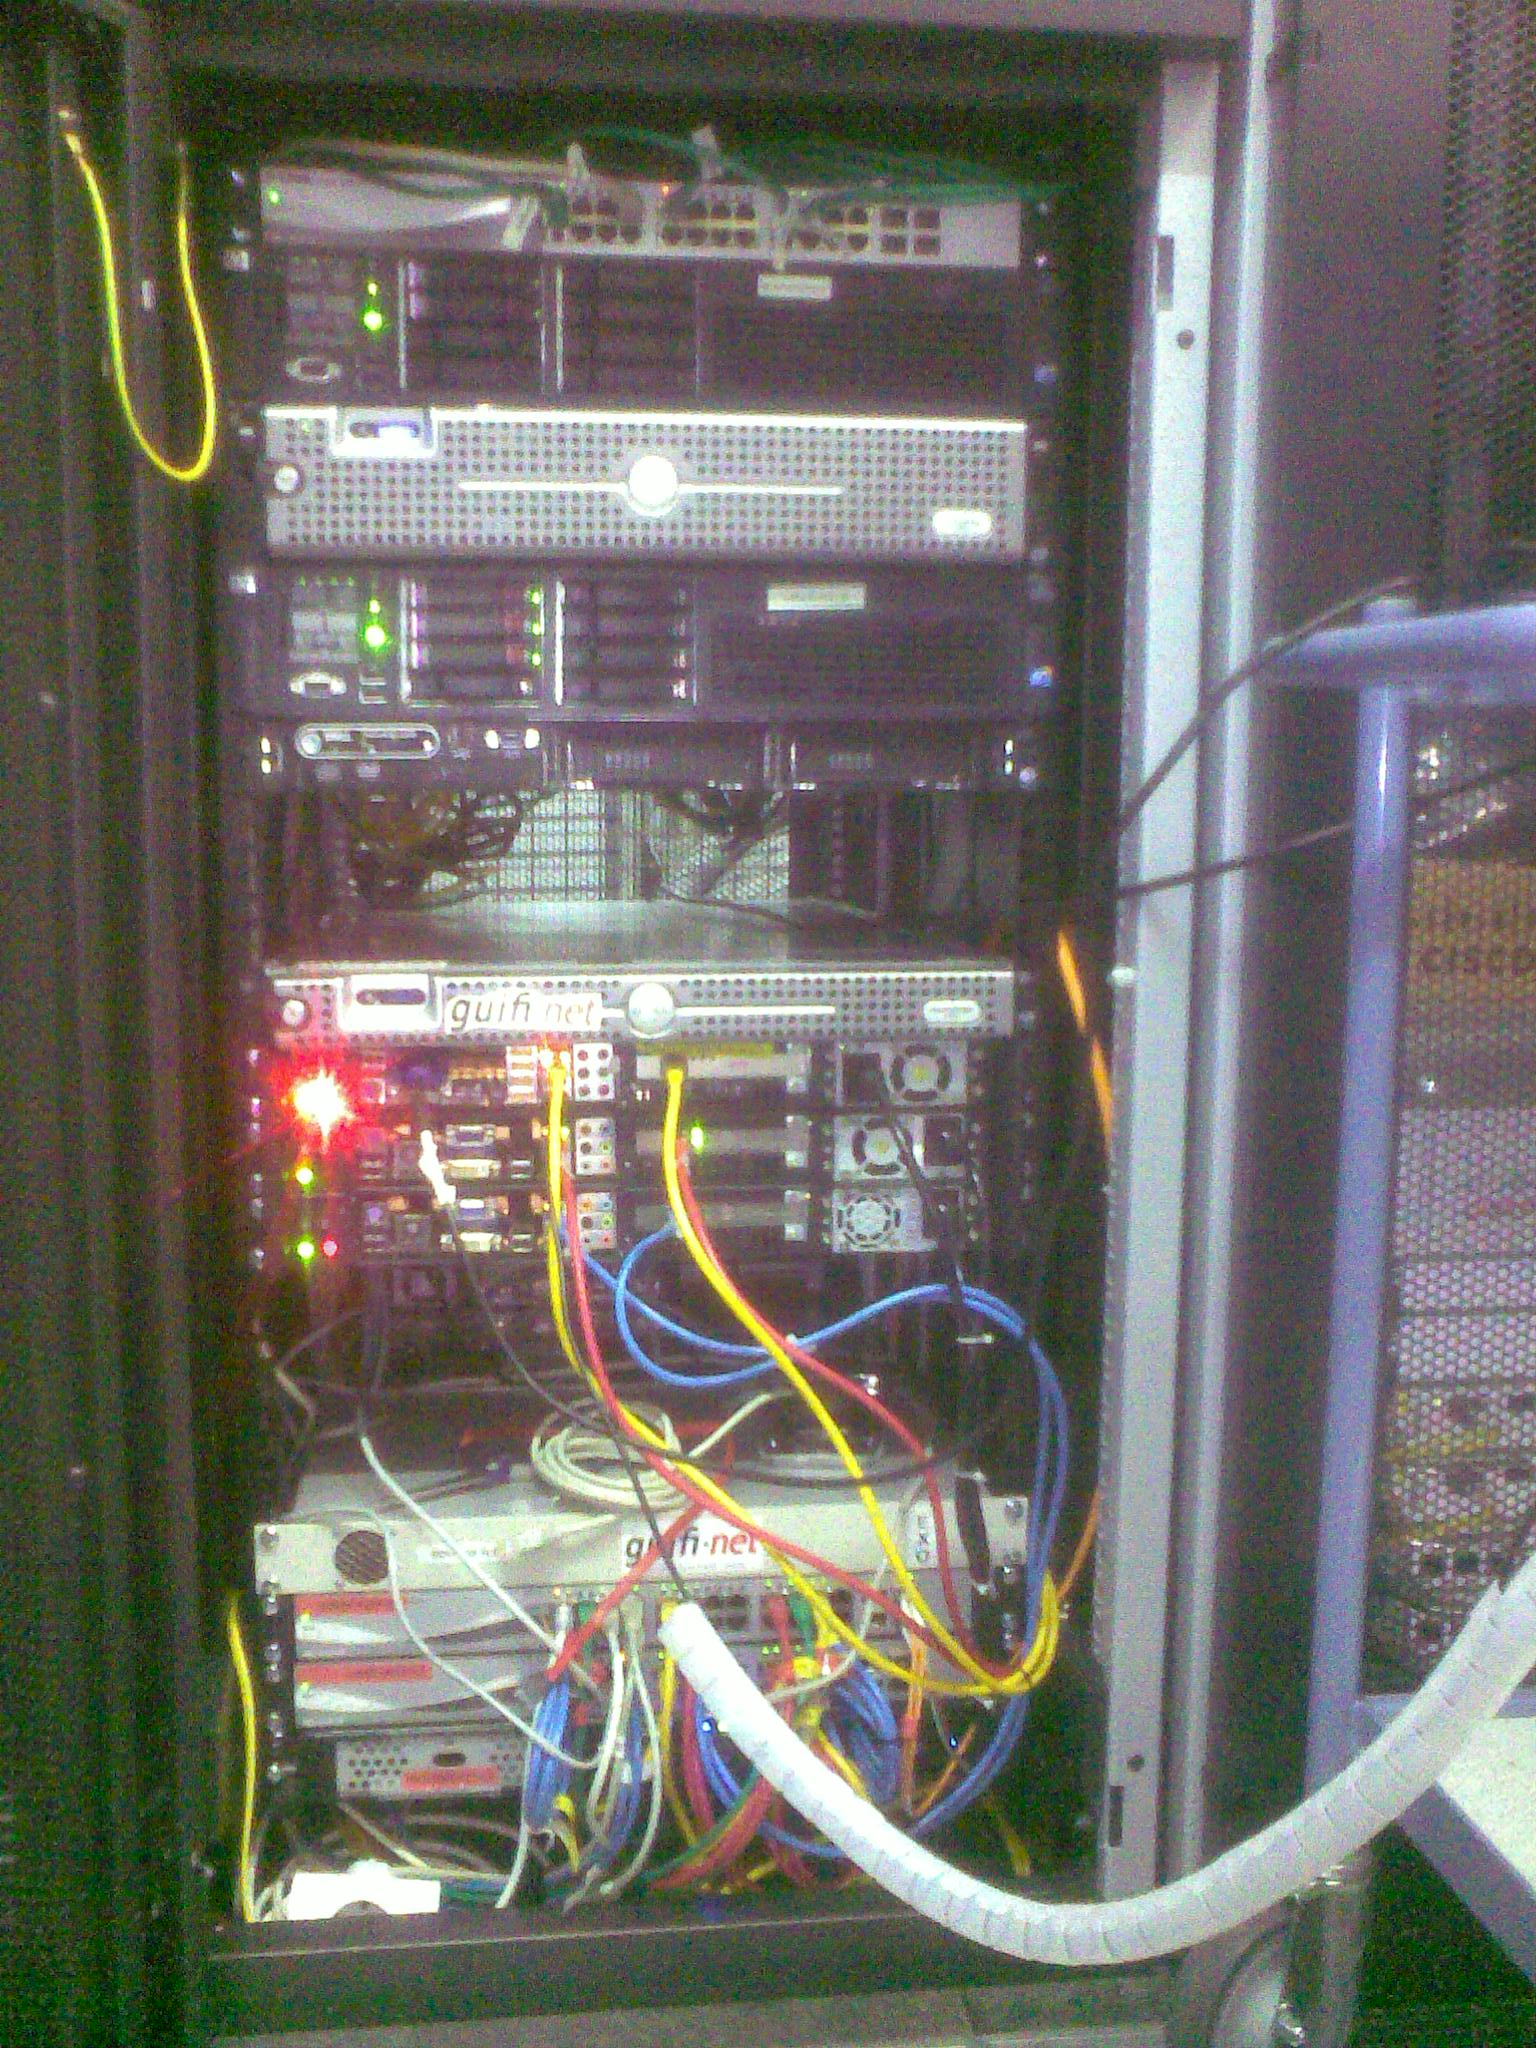
\includegraphics[scale=.65]{pops/figures/telvent_rack_front_view.eps} 
  \caption{guifi.net Foundation rack in TELVENT-Barcelona.}
  \label{fig:telvent_rack}
\end{figure}
=======
  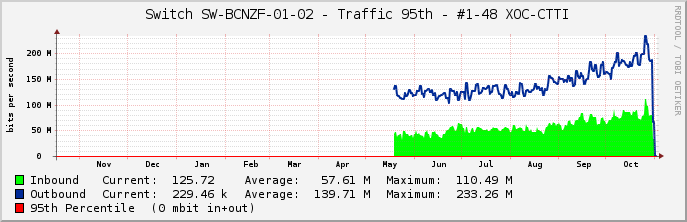
\includegraphics[width=0.95\linewidth]{sect3/figures/gurb.png} 
  \caption[Gurb PoP traffic 2013]{Gurb PoP traffic 2013.}
  \label{fig:gurb_transit}
\end{figure}


\FloatBarrier
\subsubsection{Vic}
\label{pop_vic}
>>>>>>> rbaig/master:D_5_4_2_report_on_pilots_on_fiber_deployment_b/sect3/pops.tex

As already foreseen in the previous report, this PoP was activated few days after the report was realised. Despite the fact that Vic borders Gurb, This PoP was raised as an alternative to the impossibility of reaching the Gurb's PoP. The equipment is allocated in a data centre of a facilitate of the local government (http://www.vitvic.cat/). Firgure~\ref{fig:vic_transit} shows the transit of this PoP.

\begin{figure}[H]
  \centering
<<<<<<< HEAD:D_5_4_2_report_on_pilots_on_fiber_deployment_b/pops/pops.tex
  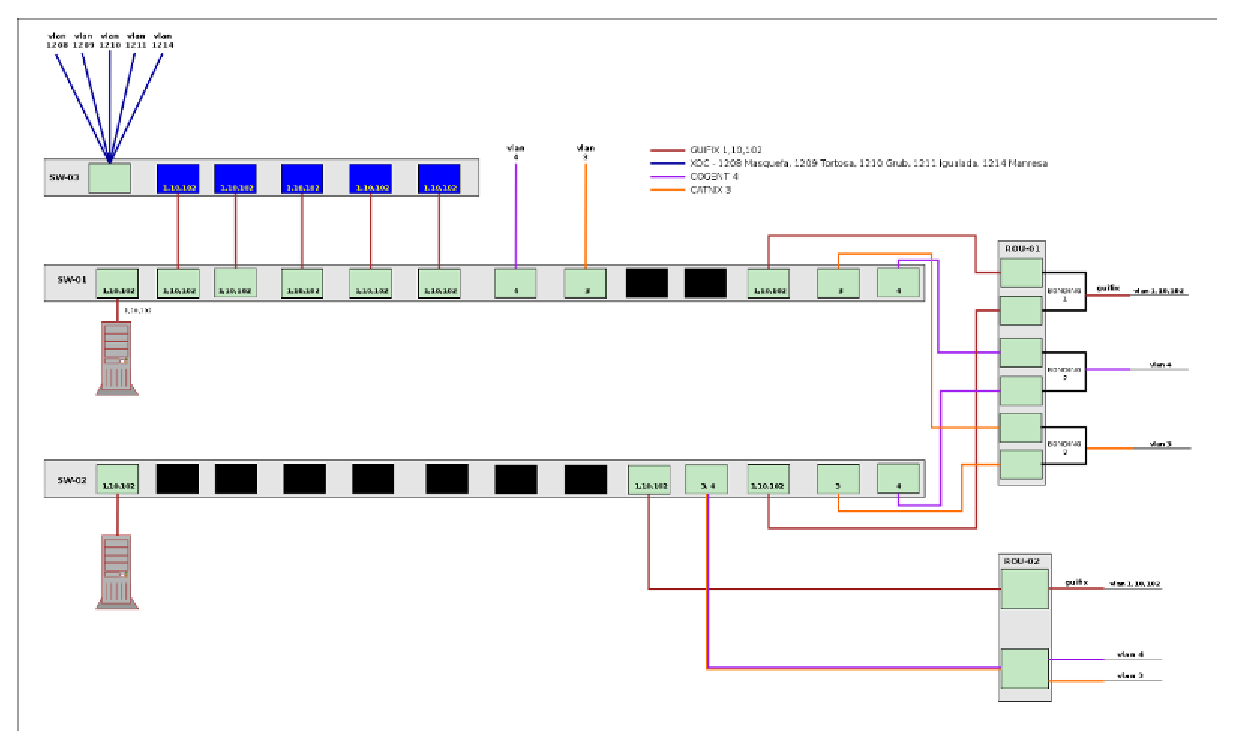
\includegraphics[scale=.75]{pops/figures/telvent_scheme.eps} 
  \caption{CATNIX connections scheme}
  \label{fig:telvent_scheme}
=======
  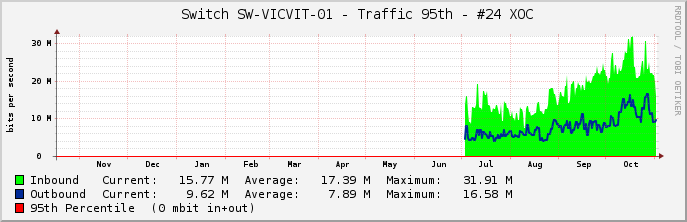
\includegraphics[width=0.95\linewidth]{sect3/figures/vic.png} 
  \caption[Vic PoP traffic 2013]{Vic PoP traffic 2013.}
  \label{fig:vic_transit}
>>>>>>> rbaig/master:D_5_4_2_report_on_pilots_on_fiber_deployment_b/sect3/pops.tex
\end{figure}


\FloatBarrier
\subsubsection{Rub\'{i}}
\label{pop_rubi}

In contrast to Vic, where due to its proximity to Gurb the option of not raising a PoP was worked, Rubí pilot clearly needs its own PoP. Thus, if the pilot is eventually developed in 2014 this PoP must be raised.


\FloatBarrier
\subsection{Other POPs}
\label{pop_others}

Firgure~\ref{fig:others_transit} shows the transit of the rest of the operational territorial PoPs .


\begin{figure}[H]
  \centering
    \begin{tabular}{c}
      \resizebox{0.75\linewidth}{!}{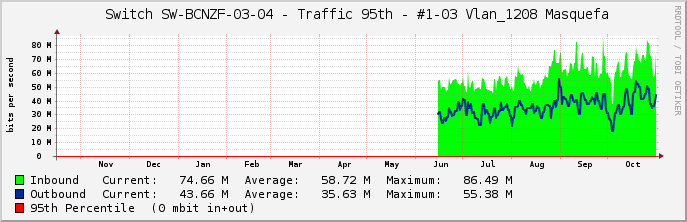
\includegraphics{sect3/figures/masquefa.png}} \\
      \resizebox{0.75\linewidth}{!}{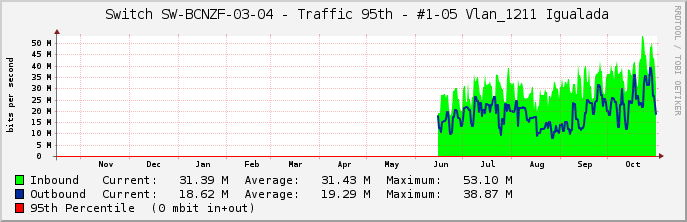
\includegraphics{sect3/figures/igualada.png}} \\
      \resizebox{0.75\linewidth}{!}{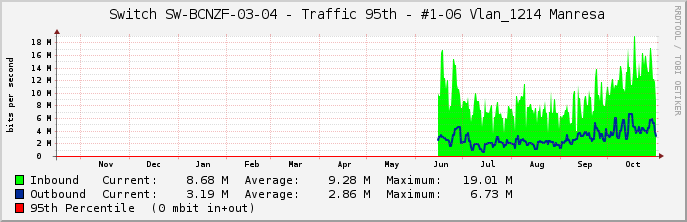
\includegraphics{sect3/figures/manresa.png}} \\
      \resizebox{0.75\linewidth}{!}{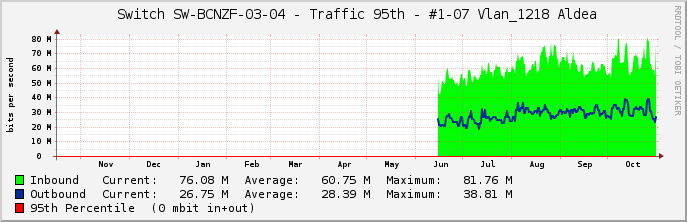
\includegraphics{sect3/figures/aldea.png}} \\
      \resizebox{0.75\linewidth}{!}{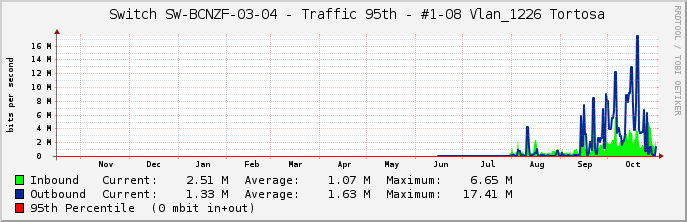
\includegraphics{sect3/figures/tortosa.png}} \\
    \end{tabular}
  \caption[Other PoPs traffic 2013]{Other PoPs traffic 2013. Top: Masquefa. Second top: Igualda. Middle: Manresa. Second bottom: Aldea. Bottom: Tortosa.}
  \label{fig:others_transit}
\end{figure}

%\item Masquefa
%\item Igualda
%\item Manresa
%\item Aldea
%\item Tortosa
